\chapter{Fundamentação Teorica}\label{cap:Fundamentação Teorica}

Esse trabalho é desenvolvido a partir  do estudo dos conceitos fundamentais de dinâmica e controle de veículos espaciais. Nas seções a seguir são apresentados os elementos teóricos para a fundamentação da modelagem física e matemática, da trajetória de um veículo espacial em uma órbita circular, da dinâmica de rotacional de um corpo rígido e do controle proporcional, integral e derivativo .

\section{Sistemas de Coordenadas e medida do tempo}

É de fundamental importância para qualquer estudo da mecânica a determinação objetiva dos sistemas de referência, sendo eles o de coordenadas e o de tempo. O parâmetro para essa escolha é a facilitação da formulação, visualização e análise.  

\subsection{Sistema de coordenadas geocêntrico-equatorial inercial }

Esse sistema quando assumido que não é rotacional e fixo no espaço é compreendido como inercial. A origem de seus eixos $X_{SCGI}$, $Y_{SCGI}$, $Z_{SCGI}$, se encontra fixo no centro de massa da Terra, ou seja geocêntrico.

O eixo $X_{SCGI}$ tem como sentido o equinócio vernal $\Upsilon$, o eixo $Z_{SCGI}$ aponta para a normal do plano equatorial terrestre, ou seja, para o polo Norte celeste e o eixo $Y_{SCGI}$ completa a base ortogonal dextrogiro. Mostrado na Figura~\ref{fig:log}, 

\begin{figure}[htpb]
   \center
   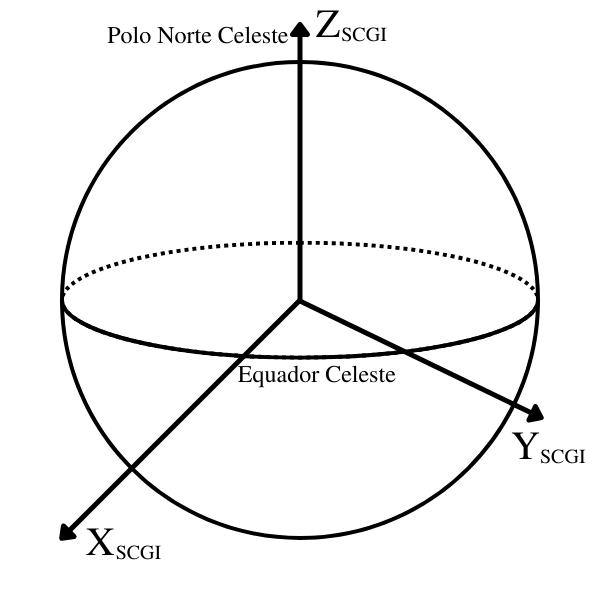
\includegraphics[scale=0.75]{figs/SCGI.PNG}
   \caption{Sistema de coordenadas geocêntrico-equatorial}
   \label{fig:log}
   \text{Fonte: Adaptada de "Fundamentals of Astrodynamics", Wertz, 1972}
\end{figure}

Esses eixos são determinados pela data de referência J2000 que é definido pela data Juliana referente ao dia 1º de Janeiro de 2000 as 12:00 tempo terrestre.

\subsection{Sistema de coordenadas orbital}

Esse sistema tem como origem o centro de massa do veículo espacial e seus eixos, $X_{SCO}$, $Y_{SCO}$, $Z_{SCO}$, acompanham sua órbita. O eixo $Z_{SCO}$ aponta em direção ao centro de massa da Terra ou, direção nominal do nadir. O eixo $Y_{SCO}$ tem como direção o oposto do vetor do plano de órbita do veiculo espacial. E o eixo $X_{SCO}$ aponta para o vetor velocidade ou, trajetória da órbita. Representado Figura~\ref{fig:log},

\subsection{Sistema de coordenadas fixo no corpo}

\section{Mecânica Orbital}
\subsection{Problema de dois corpos}
\subsection{Determinação dos elementos orbitais pelos vetores posição e velocidade}

\section{Dinâmica de Atitude}
\subsection{Matriz de cossenos diretores}
\subsection{Ângulos de Euler}
\subsection{Eixo-Angulo de Euler}
\subsection{Parâmetros de Euler - Quatérnions}
\subsection{Equações Diferenciais da Cinemática}
\subsection{Formulação Geral da Dinâmica de Corpo Rígido}
\subsection{Corpo Rígido em Órbita Circular}

\section{Determinação e Controle de Atitude}
\subsection{Algorítimo TRIAD}
\subsection{Filtro de Kalman}
\subsection{Técnica de Controle Proporcional Integral Derivativa}
